\documentclass{article}
\usepackage{graphicx}
\usepackage{amssymb,amsmath}
\usepackage{tikz}
\usetikzlibrary{arrows}

\author{Stefano Duca \and Alexandros Rigos}
\title{Contracts in an Evolutionary Prisoner's Dilemma Game: A Report}

\begin{document}

\maketitle

\section{The main idea}
Here we are playing what we call a contract game in a prisoner's dilemma on a spatial lattice.

The idea is that a player can offer a part of what he earns ($\Delta$) to the other player to make it convienent to cooperate, conditional on the event of both players cooperating. Of course he might be tempted to defect but, due to the preference of errors, maybe the cooperation will be stable.

Here is the payoff matrix of the game:
%\begin{table}
%\centering
\begin{center}
\begin{tabular}{|c|c|c|c|}
\hline 
• & C & D & Delta \\ 
\hline 
C & r,r & -a,1 & r+$\Delta$, r-$\Delta$ \\ 
\hline 
D & 1,-a & 0,0 & 1, -a \\ 
\hline 
Delta & r- $\Delta$, r+$\Delta$ & -a, 1 & r,r, \\ 
\hline 
\end{tabular} 
\end{center}
%\end{table}

The player play a logit best response with parameter delta, responding to the strategy array of the previous round.

We implement the idea in several different ways:

Logit best response

\subsection{Logit best response with 4 strategies and directional transitions}
We now introduce another strategy: -Delta. Players that use this strategy, if their opponent cooperates, will take a larger part of the pie. More specifically, they will get $r+\Delta$ and their opponent will receive $r-\Delta$. The payoff matrix is, therefore amended to be the following:
\begin{center}
\begin{tabular}{|c|c|c|c|c|}
\hline 
• & C & D &+Delta & -Delta  \\ 
\hline 
C & $r$ , $r$ & $-a$ , 1 & $r+\Delta$, $r-\Delta$ & $r-\Delta$, $r+\Delta$ \\ 
\hline 
D & 1 , $-a$ & 0,0 & 1, $-a$ & 1,$-a$\\ 
\hline 
+Delta & $r -\Delta$, $r+\Delta$ & $-a$, 1 & $r$ , $r$& $r-2\Delta$, $r+2\Delta$ \\ 
\hline 
-Delta & $r+\Delta$ , $r-\Delta$ & $-a$, 1 & $r+2\Delta$ , $r-2\Delta$ & $r$ ,$ r$\\ 
\hline 
\end{tabular} 
\end{center}

Similarly as in previous cases, there is a logit rule in the way that agents switch stratetegies. Crucially, we allow only for specific transitions to tale place. These are shown in the following diagram. An arrow indicates a transition that is allowed. 

\begin{center}
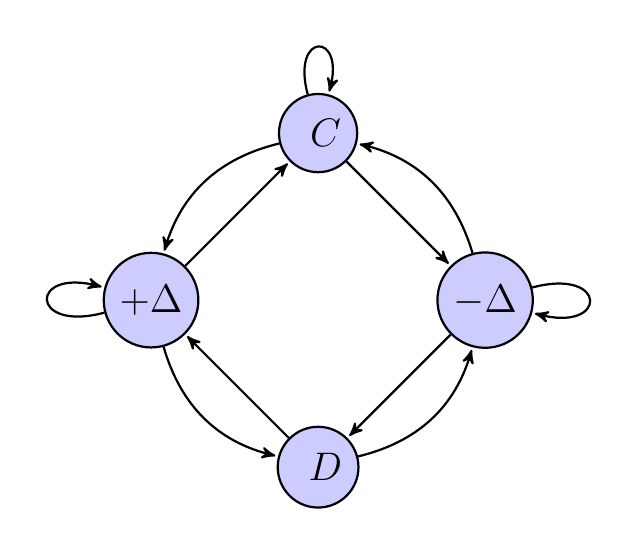
\begin{tikzpicture}[->,>=stealth',shorten >=1pt,auto,node distance=3cm,
  thick,main node/.style={circle,fill=blue!20,draw,font=\sffamily\Large\bfseries}]
  \node[main node] (1) {$~C$};
  \node[main node] (2) [below left of=1] {$+\Delta$};
  \node[main node] (3) [below right of=2] {$~D$};
  \node[main node] (4) [below right of=1] {$-\Delta$};

  \path[every node/.style={font=\sffamily\small}]
    (1) edge node [left] { } (4)
        edge [bend right] node[left] { } (2)
        edge [loop above] node { } (1)
    (2) edge node [right] { } (1)
	%edge node {} (4)
        edge [loop left] node {} (2)
        edge [bend right] node[left] {} (3)
    (3) edge node [right] {} (2)
        edge [bend right] node[right] {} (4)
    (4) edge node [left] {} (3)
        edge [loop right] node {} (4)
        edge [bend right] node[right] {} (1);
\end{tikzpicture}
\end{center}

Results show that the directional transitions do not change the percentage of cooperators in the long run (see the following figures).

Imitation

Imitation with delta conditional on last round's decisions.

\section{Future}

\subsection{Best responders with imitators}

\section{other ideas}
group scoring with stars and intermediate rounds of interaction
%\section{Notes on the code}
%\begin{enumerate}
%\item  So far we consider 3 types of lattice:
%0 stands for squared lattice with Von Neumann n.n. ;
%1 stands for squared lattice with Moore n.n.;
%2 stands for ring lattice.

%\item 0 is C, 1 is D and 2 is Delta
%\end{enumerate}

\end{document}
